\subsection{Datenmodell einer Klassifikation}
    \label{section:solutionDetailsPersistenceDataModel}
    Die Struktur der Graphen im {\classificationStorage} unterscheidet
    sich von den bisher vorgestellten Datenmodellen.
    Die Beschreibung dieser Struktur geht zunächst auf die Entitäten ein,
    die Knoten im Graphen darstellen.
    Anschließend folgt die Betrachtung der Beziehungen.
    Abbildung \ref{image:dbDataModelOverview} zeigt zur Veranschaulichung
    der Ausführungen eine Übersicht des Datenmodells.

    \begin{figure}
        \centering
        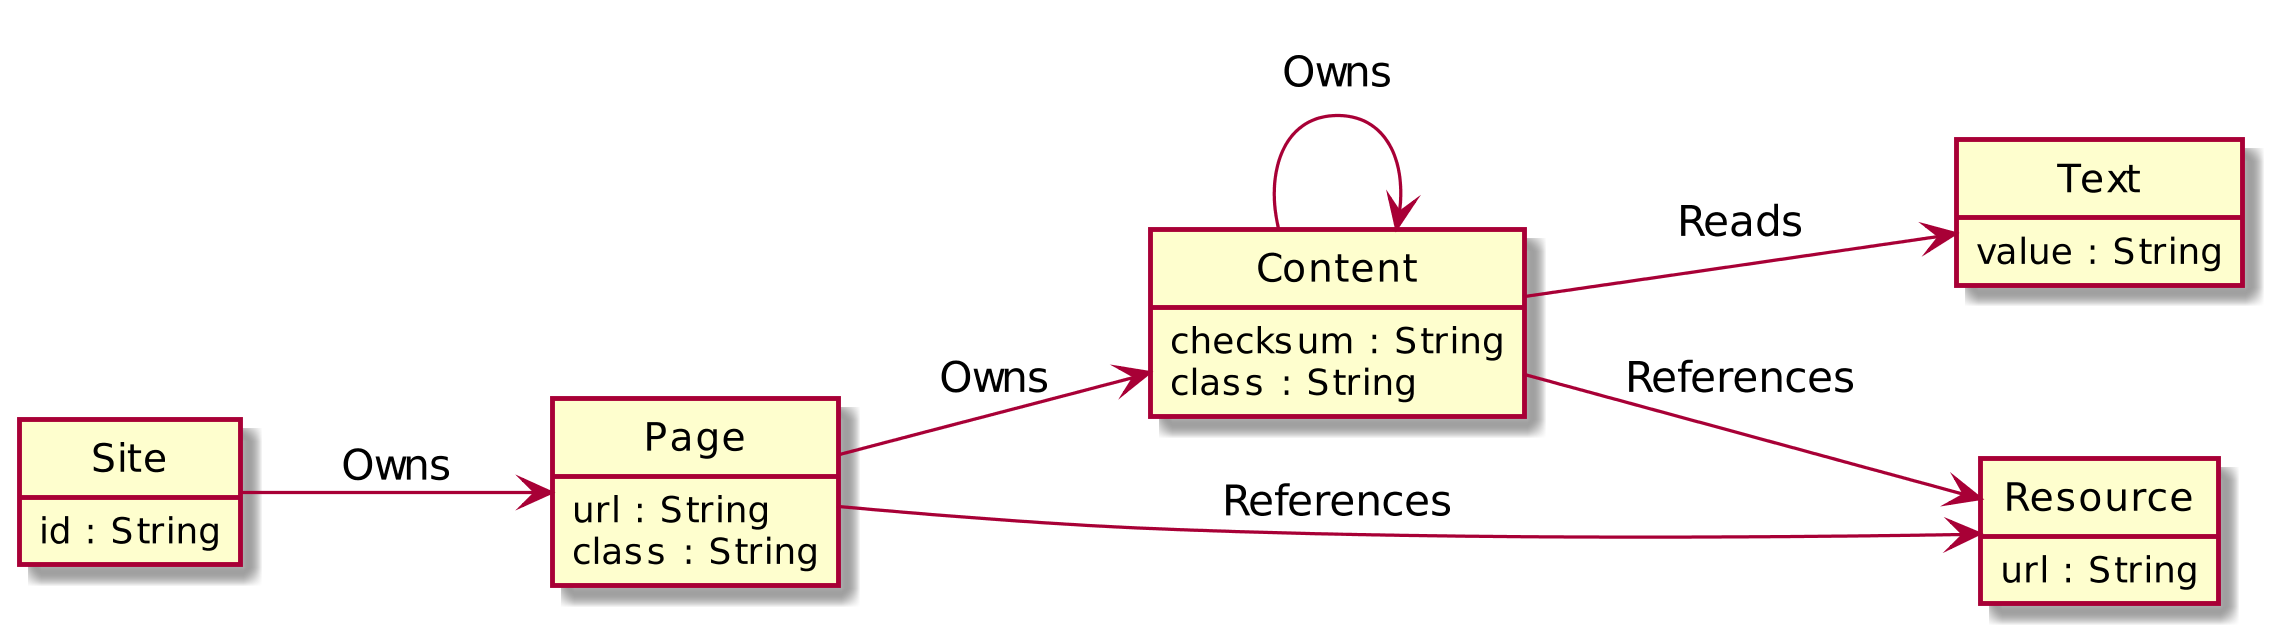
\includegraphics[scale=\imageScalingFactor]{../resources/db-data-model/nodes.png}
        \caption{Das Datenmodell einer Klassifikation im {\classificationStorage}}
        \label{image:dbDataModelOverview}
    \end{figure}

    \paragraph{Knoten}
    Tabelle \ref{image:solutionDetailsPersistenceEntities} zeigt,
    welche Entitäten einer Klassifikation als Knoten in der Datenbank dargestellt werden
    und welche Labels diese Knoten erhalten.
    Eine Ausnahme stellen Seiten dar,
    da sie erst als referenzierte {\resources} in die Datenbank aufgenommen werden können,
    bevor sie selbst einer Klassifizierung unterzogen werden.
    In diesem Fall erhält die Seite erst das Label \texttt{Resource} und anschließend zusätzlich
    das Label \texttt{Page}.

    \begin{table}[htb]
        \centering
        \begin{tabular}{|l|l|}
            \hline
            \textbf{Entität}                         & \textbf{Label} \\ \hline
            Seite                                    & \texttt{Page}           \\ \hline
            {\contentFeature}                        & \texttt{Content}        \\ \hline
            Textueller Inhalt eines {\contentFeature}s & \texttt{Text}         \\ \hline
            Referenzierte {\resource}                & \texttt{Resource}       \\ \hline
            Site                                     & \texttt{Site}           \\ \hline
        \end{tabular}
        \caption{Die Abbildung von Entitäten der Domäne im Graphen des {\classificationStorage}s}
        \label{image:solutionDetailsPersistenceEntities}
    \end{table}

    Sites werden durch Knoten mit dem gleichnamigen Label gespeichert und enthalten lediglich einen
    Kennzeichner, der sie identifiziert.
    Ein Seitenknoten speichert neben der Klasse der Seite auch ihre \gls{url},
    die ihn innerhalb der Datenbank eindeutig kennzeichnet.
    Der Knoten einer {\resource} enthält lediglich ihre \gls{url}, die auch hier diese Rolle einnimmt.
    Im Falle von {\contentFeature}s besitzt jedes {\scalarFeature} und jedes Element eines {\collectionFeature}s
    im Graphen einen Knoten mit dem Label \texttt{Content}.
    Diese enthalten neben der Klasse des Features eine Prüfsumme über das Feature,
    die innerhalb der Datenbank als Schlüssel solcher Knoten fungiert.
    Das Schreiben einer Klassifikation macht diese Eigenschaft ebenfalls erforderlich,
    was später behandelt wird\footnote{vgl. Kapitel \ref{section:solutionDetailsClassificationStorageAPIUpdatePage}}.
    Der Text eines {\contentFeature}s wird hingegen in einem separaten Knoten mit dem Label \texttt{Text} gespeichert,
    der neben dieser Information nichts speichert und deshalb auch eindeutig über den Text identifiziert werden kann.
    Der Grund für die Auslagerung des Textes ist, dass es viele Features geben kann, die den gleichen textuellen Inhalt besitzen.
    Diese Eigenschaft soll der Graph durch Beziehungen explizit machen,
    sodass sie leicht für Analysen genutzt werden kann.
    Eine Beziehung ist semantisch ausdrucksstärker als ein identischer Wert einer Eigenschaft mehrerer Knoten.
    Die Auswertung ist zugleich effizienter als ein Vergleich aller Knoten bzgl. einer solchen Eigenschaft.

    \paragraph{Kanten}
    Seiten und {\contentFeature}s sind in der Lage {\contentFeature}s zu enthalten.
    In der Datenbank ist ein \texttt{Page}-Knoten mit all seinen \texttt{Content}-Knoten
    durch eine Beziehung mit dem Label \texttt{Owns} verbunden.
    Das Gleiche gilt für \texttt{Content}-Knoten und ihre {\childFeature}s.
    Eine genauere Darstellung dieser Beziehung bietet Abbildung \ref{image:dbDataModelContentRelationship},
    in der sie als \texttt{FeatureRelationship} modelliert wird.

    \begin{figure}
        \centering
        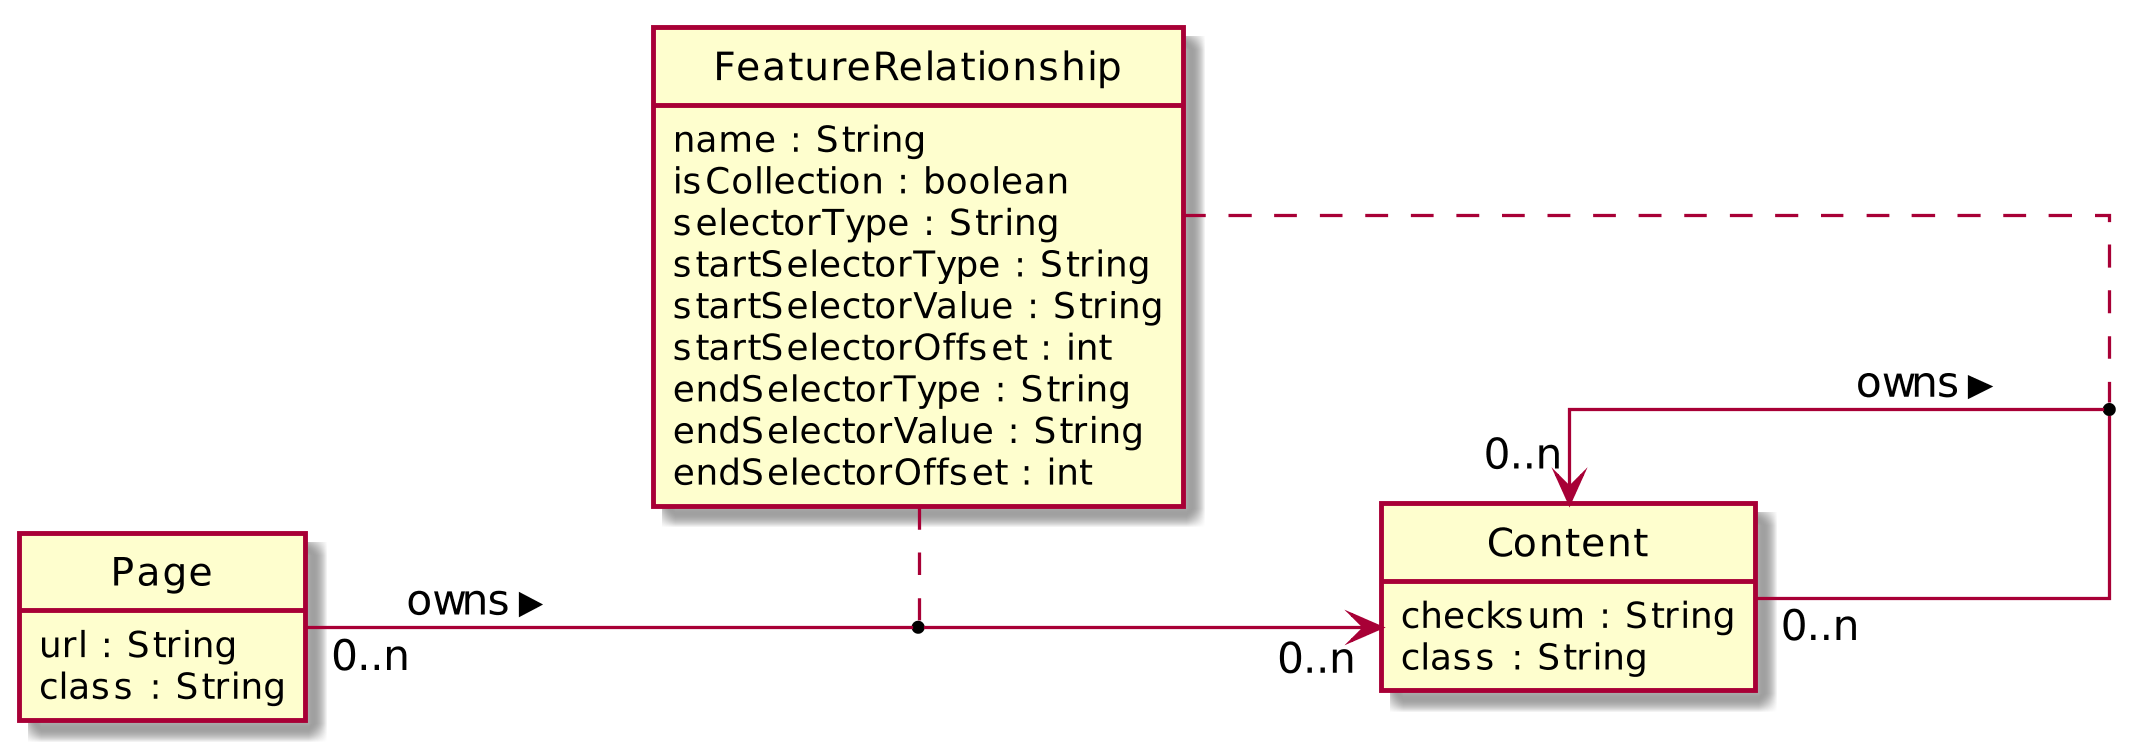
\includegraphics[scale=\imageScalingFactor]{../resources/db-data-model/content-relationship.png}
        \caption{Die Beziehung zu einem Content-Knoten}
        \label{image:dbDataModelContentRelationship}
    \end{figure}

    Die Beziehung speichert eine Reihe an Informationen.
    Neben dem Namen des Features und der Angabe,
    ob es sich um ein Element eines {\collectionFeature}s handelt,
    sind dies die Bestandteile des eindeutigen Selektors des
    klassifizierten Elementes.
    Obwohl die beiden XPath-Ausdrücke identisch sind,
    werden sie einzeln in der Beziehung gespeichert, damit das Datenmodell der Datenbank
    nicht angepasst werden muss, falls diese Prämisse in Zukunft ungültig wird.
    Im Falle eines {\collectionFeature}s hat ein Knoten pro Element des Features eine solche
    ausgehende Kante, die alle den gemeinsamen Namen des Features speichern.
    Wie später gezeigt wird, ist es sinnvoll diese Informationen nicht im \texttt{Content}-Knoten
    zu speichern, um ihre Wiederverwendbarkeit zu
    steigern\footnote{vgl. Kapitel \ref{section:solutionDetailsClassificationStorageAPIUpdatePage}}.
    Referenzen werden in der Datenbank durch eine Kombination aus
    \texttt{Resource}-Knoten und Beziehungen zu diesen Knoten dargestellt.
    Diese Beziehungen tragen das Label \texttt{References}.
    Abbildung \ref{image:dbDataModelResourceRelationship} stellt diese Beziehung in den Fokus.

    \begin{figure}
        \centering
        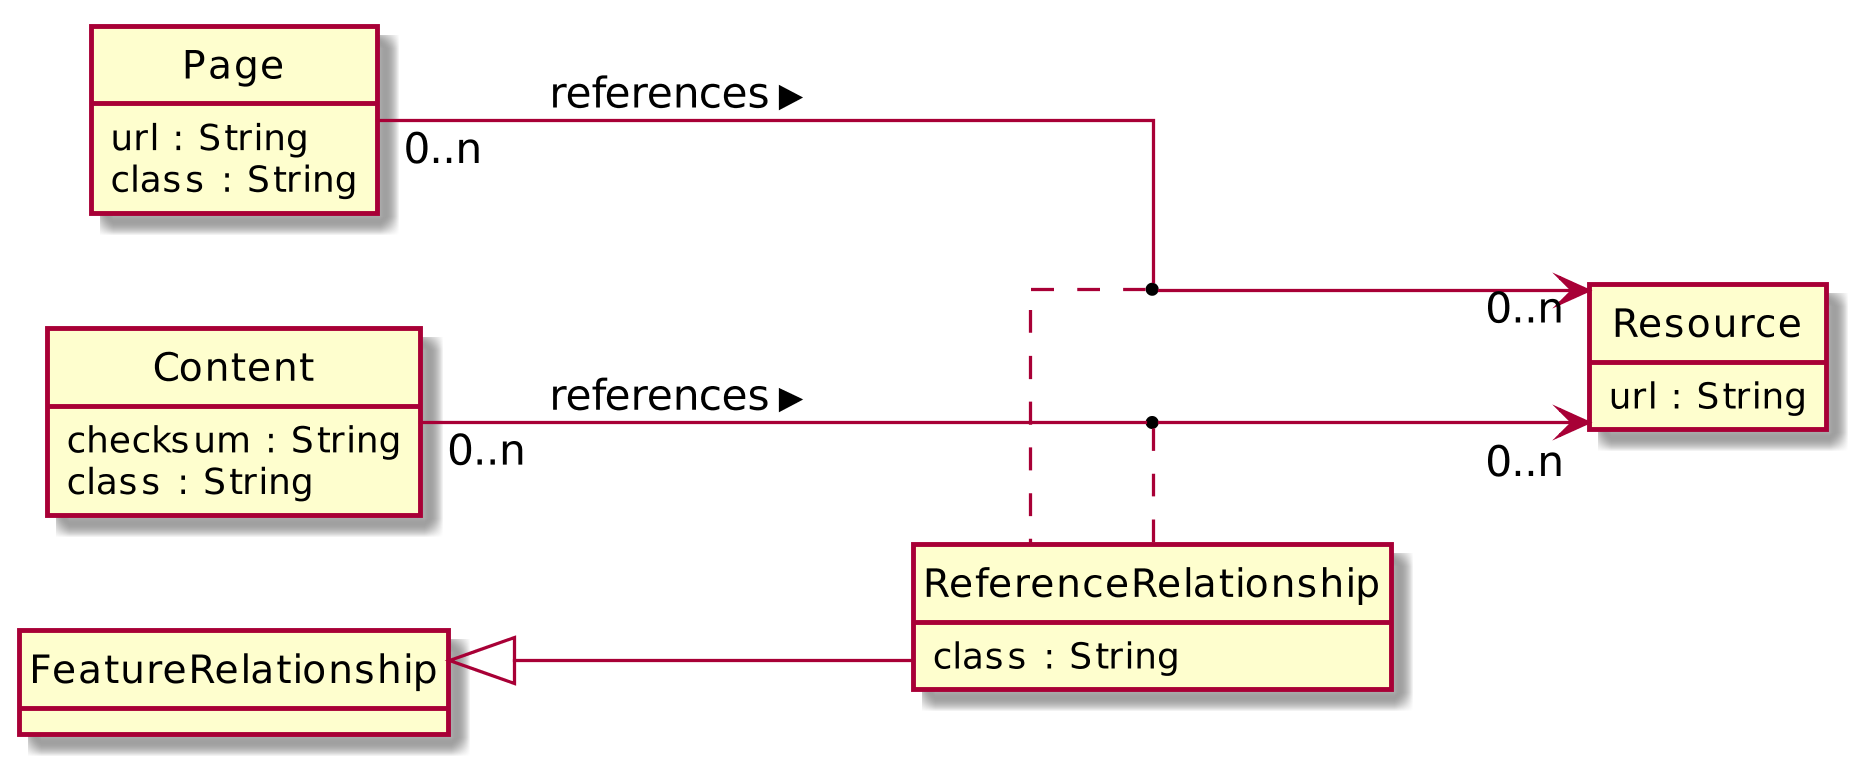
\includegraphics[scale=\imageScalingFactor]{../resources/db-data-model/resource-relationship.png}
        \caption{Die Beziehung zu einem {\resource}-Knoten}
        \label{image:dbDataModelResourceRelationship}
    \end{figure}

    Wie zu sehen ist, handelt es sich bei einer solchen \texttt{ReferenceRelationship} ebenfalls
    um eine \texttt{FeatureRelationship}, weshalb sie die oben beschriebenen Informationen speichert.
    Zusätzlich enthält sie aber auch die Klasse des {\referenceFeature}s.
    Diese kann nicht im \texttt{Resource}-Knoten gespeichert werden,
    weil er Ziel vieler Referenzen mit unterschiedlichen Klassen sein kann.
    Besitzt ein {\contentFeature} textuellen Inhalt,
    ist der entsprechende \texttt{Content}-Knoten über eine \texttt{Reads}-Beziehung
    mit einem \texttt{Text}-Knoten verbunden.
    Durch \texttt{Owns}-Kanten modellieren \texttt{Site}-Knoten,
    welche Seiten ihnen angehören.
